\subsubsection{Rationale/Context}
In order to travel, every traveller has to buy a ticket. This can be done in two ways, either by going to the office of the Ferry Service or by buying a ticket online through the new system. 
\subsubsection{User story}
As a \textit{traveller}, I want to \textit{buy a ticket}, from a given origin to a given destination.
\subsubsection{Use Case}
\creator{\studentA}
\updater{\studentB}
\secondUpdater{\studentC}

\textbf{Use Case Name:} Create a ticket

\textbf{Scope:} Tickets buying system

\textbf{Level:} User Goal

\textbf{Primary Actor:} Commuter

\textbf{Stakeholders and Interests:} 
\begin{itemize}
\item \textit{Commuter:} Wants to buy a ticket quickly through the website, without having to go to the office.
\item \textit{Seller:} Wants the ticket purchasing process to become automated, thus to have less paperwork and less manual work.
\end{itemize}

\textbf{Preconditions:}
\begin{itemize}
\item The user is authenticated on the website and his account is confirmed.
\end{itemize}

\textbf{Success Guarantee (Postconditions):}
\begin{itemize}
    \item State change: The information of ticket has been added and the information about a trip has been updated.
    \item Output: A .pdf file containing the e-ticket shown to the screen and sent to the traveller's email address.
\end{itemize}

\textbf{Main Success Scenario (Basic Flow):}
\begin{enumerate}
\item The User indicates to the System, the wish to buy a ticket.
\item The System sends the User a ticket customisation form with available departure/return dates and times.
\item The User fills in the form: the number of passengers, the number of bikes and dogs, the type of ferry, the origin, and the destination.
\item The User sends the System the filled-in ticket selection form.
\item The System checks whether the form is completed correctly (i.e., complete and error-free).
\item The System informs the User about its findings ("Ok" or indicating the gaps and errors found).
\item If the form is not completed correctly, steps 3 - 6 will be repeated.
\item The System sends the User a payment method form with possible payment methods.
\item The User fills in the form: payment method.
\item The User sends the System the filled-in payment method form.
\item The System checks whether the form is completed correctly (i.e., complete).
\item The System informs the User about its findings ("Ok" or indicating the gaps and errors found).
\item If the form is not completed correctly, steps 9 - 12 will be repeated.
\item The System executes a transaction using the given payment method.
\item The System generates a new, unique ticket code.
\item The System stores all the information about the ticket.
\item The System generates an e-ticket and shows it to the screen.
\item The System sends the User an email address input form.
\item The User fills in the form with his email address.
\item The User sends the System the filled-in email input form.
\item The System checks whether the form is completed correctly (i.e., complete and error-free).
\item The System informs the User about its findings ("Ok" or indicating a syntax error in the introduced email address).
\item If the form is not completed correctly, steps 19 - 22 will be repeated.
\item The System sends the ticket the user's email address.
\end{enumerate}
Extensions:
\begin{enumerate}
    \item[6a.1.] If there is more than one bike per person, the System will notify the user.
    \item[] \phantom{x}
    
    \item[13a.1.] If the user has chosen iDEAL in the form at step 9, the System sends the User a form containing the possible banks.
    \item[13a.2.] The User chooses the preferred bank.
    \item[13a.3.] The User sends the System the filled-in payment information form.
    \item[13a.4.] The System checks whether the form is completed correctly (i.e., complete and error-free).
    \item[13a.5.] The System informs the User about its findings ("Ok" or indicating the gaps and errors found).
    \item[13a.6.] If the form is not completed correctly, steps 13a.2 - 13a.5 will be repeated.
    \item[] \phantom{x}
    
    \item[13b.1.] If the user has chosen credit card payment in the form at step 9, the System sends the User a form containing the credit card holder, the credit card expiration date, the credit card number.
    \item[13b.2.] The User fills in: the credit card holder, the credit card expiration date, the credit card number.
    \item[13b.3.] The User sends the System the filled-in payment information form.
    \item[13b.4.] The System checks whether the form is completed correctly (i.e., complete and error-free).
    \item[13b.5.] The System informs the User about its findings ("Ok" or indicating the gaps and errors found).
    \item[13b.6.] If the credit card number and/or expiration date is not valid, the System will inform the User.
    \item[13b.7.] If the form is not completed correctly, steps 13b.2 - 13b.6 will be repeated.
    \item[] \phantom{x}
    
    \item[14a.] If the transaction fails, then the System show the reason of the error to the User and returns him to the payment information form.
\end{enumerate}

\textbf{Technology And Data Variations List:} 
\begin{itemize}
    \item Cardholder name: String with alphabetical characters only
    \item Departure and return date: Date of the form DD/MM/YYYY
    \item Card expiration date: Date of the form MM/YYYY
    \item Number of bikes and dogs: Integer
    \item CVV card code: Three digit number
    \item Destination name, Ferry type, Bank name: String chosen from a list
    \end{itemize}

\textbf{Frequency of Occurrence:} Multiple times a day, every day.

\subsubsection{SSD}
\creator{\studentA}
\updater{\studentB}
\secondUpdater{\studentC}
Considering the previous sub-sections we can create the following SSD model:\\\\
User $\rightarrow$ System: BuyTicket;\hfill /* 1\\
System $\rightarrow$ User: Ticket selection form;\hfill /* 2\\
repeat User $\rightarrow$ User: Fill in the form with: \underline{number of passengers}, \underline{number of bikes},\\ \underline{number of dogs}, \underline{type of ferry}, \underline{destination city};\hfill /* 3\\
\phantom{x}\hspace{7mm} User $\rightarrow$ System: Filled-in Ticket selection form;\hfill /* 4\\
\phantom{x}\hspace{7mm} System $\rightarrow$ System: Check whether the form is completed correctly; \hfill /* 5\\
\phantom{x}\hspace{7mm} System $\rightarrow$ User: "Ok" or the found gaps and errors;\hfill /* 6\\
\phantom{x}\hspace{7mm} if number of bikes greater than the number of people\\
\phantom{x}\hspace{14mm} then System $\rightarrow$ User: "You can only bring one bike per person!"; \hfill /* 6a.1\\
until the form is completed correctly;\hfill /* 7\\
System $\rightarrow$ User: Payment method form;\hfill /* 8\\
repeat User $\rightarrow$ User: Fill in the payment method form with: \underline{payment method};\hfill /* 9\\
\phantom{x}\hspace{7mm} User $\rightarrow$ System: Filled-in payment form;\hfill /* 10\\
\phantom{x}\hspace{7mm} System $\rightarrow$ System: Check whether the form is completed correctly; \hfill /* 11\\
\phantom{x}\hspace{7mm} System $\rightarrow$ User: "Ok" or the found gaps and errors;\hfill /* 12\\
until the form is completed correctly;\hfill /* 13\\
if payment method is iDEAL\\
then System $\rightarrow$ User: Payment form containing the \underline{possible banks};\hfill /* 13a.1\\
\phantom{x}\hspace{7mm} repeat User $\rightarrow$ User: Fill in the bank of choice;\hfill /* 13a.2\\
\phantom{x}\hspace{14mm} User $\rightarrow$ System: Filled-in payment information form;\hfill /* 13a.3\\
\phantom{x}\hspace{14mm} System $\rightarrow$ System: Check whether the form is completed correctly; \hfill /* 13a.4\\
\phantom{x}\hspace{14mm} System $\rightarrow$ User: "Ok" or the found gaps and errors;\hfill /* 13a.5\\
\phantom{x}\hspace{7mm} until the form is completed correctly;\hfill /* 13a.6\\
else\\
\phantom{x}\hspace{7mm} System $\rightarrow$ User: Payment information form;\hfill /* 13b.1\\
\phantom{x}\hspace{7mm} repeat User $\rightarrow$ User: Fill in payment information form with credit card holder, credit card number and credit card expiration date;\hfill /* 13b.2\\
\phantom{x}\hspace{14mm} User $\rightarrow$ System: Filled-in payment information form;\hfill /* 13b.3\\
\phantom{x}\hspace{14mm} System $\rightarrow$ System: Check whether the form is completed correctly; \hfill /* 13b.4\\
\phantom{x}\hspace{14mm} System $\rightarrow$ User: "Ok" or the found gaps and errors;\hfill /* 13b.5\\
\phantom{x}\hspace{14mm} if credit card and/or expiration date not valid\\
\phantom{x}\hspace{21mm} then System $\rightarrow$ User: "Payment information not valid!";\hfill /*13b.6\\
\phantom{x}\hspace{7mm} until the form is completed correctly;\hfill /* 13b.7\\
fi\\
System $\rightarrow$ System: MakeTransaction using the payment credentials or iDeal;\hfill /* 14\\
if transaction failed\\
then System $\rightarrow$ User: Show the reason for transaction failure and restart process;\hfill /* 14a\\
else System $\rightarrow$ System: GenerateUniqueTicketNumber;\hfill /* 15\\
\phantom{x}\hspace{7mm} System $\rightarrow$ System: SaveInformation;\hfill /* 16\\
\phantom{x}\hspace{7mm} System $\rightarrow$ User: Show the generated e-ticket;\hfill /* 17\\
\phantom{x}\hspace{7mm} System $\rightarrow$ User: Email address form; \hfill /* 18\\
\phantom{x}\hspace{7mm} repeat User $\rightarrow$ User: Fill in email address form with email address; \hfill /* 19\\
\phantom{x}\hspace{14mm} User $\rightarrow$ System: Filled-in email address form;\hfill /* 20\\
\phantom{x}\hspace{14mm} System $\rightarrow$ System: Check whether the form is completed correctly; \hfill /* 21\\
\phantom{x}\hspace{14mm} System $\rightarrow$ User: "Ok" or the found gaps and errors in the email address;\hfill /* 22\\
\phantom{x}\hspace{7mm} until the form is completed correctly;\hfill /* 23\\
\phantom{x}\hspace{7mm} System $\rightarrow$ User: Send the generated e-ticket to the user's email; \hfill /* 24\\
fi

\subsubsection{Grey box SD}
\creator{\studentC}
\updater{\studentA}
\begin{lrbox}{\mysavebox}%
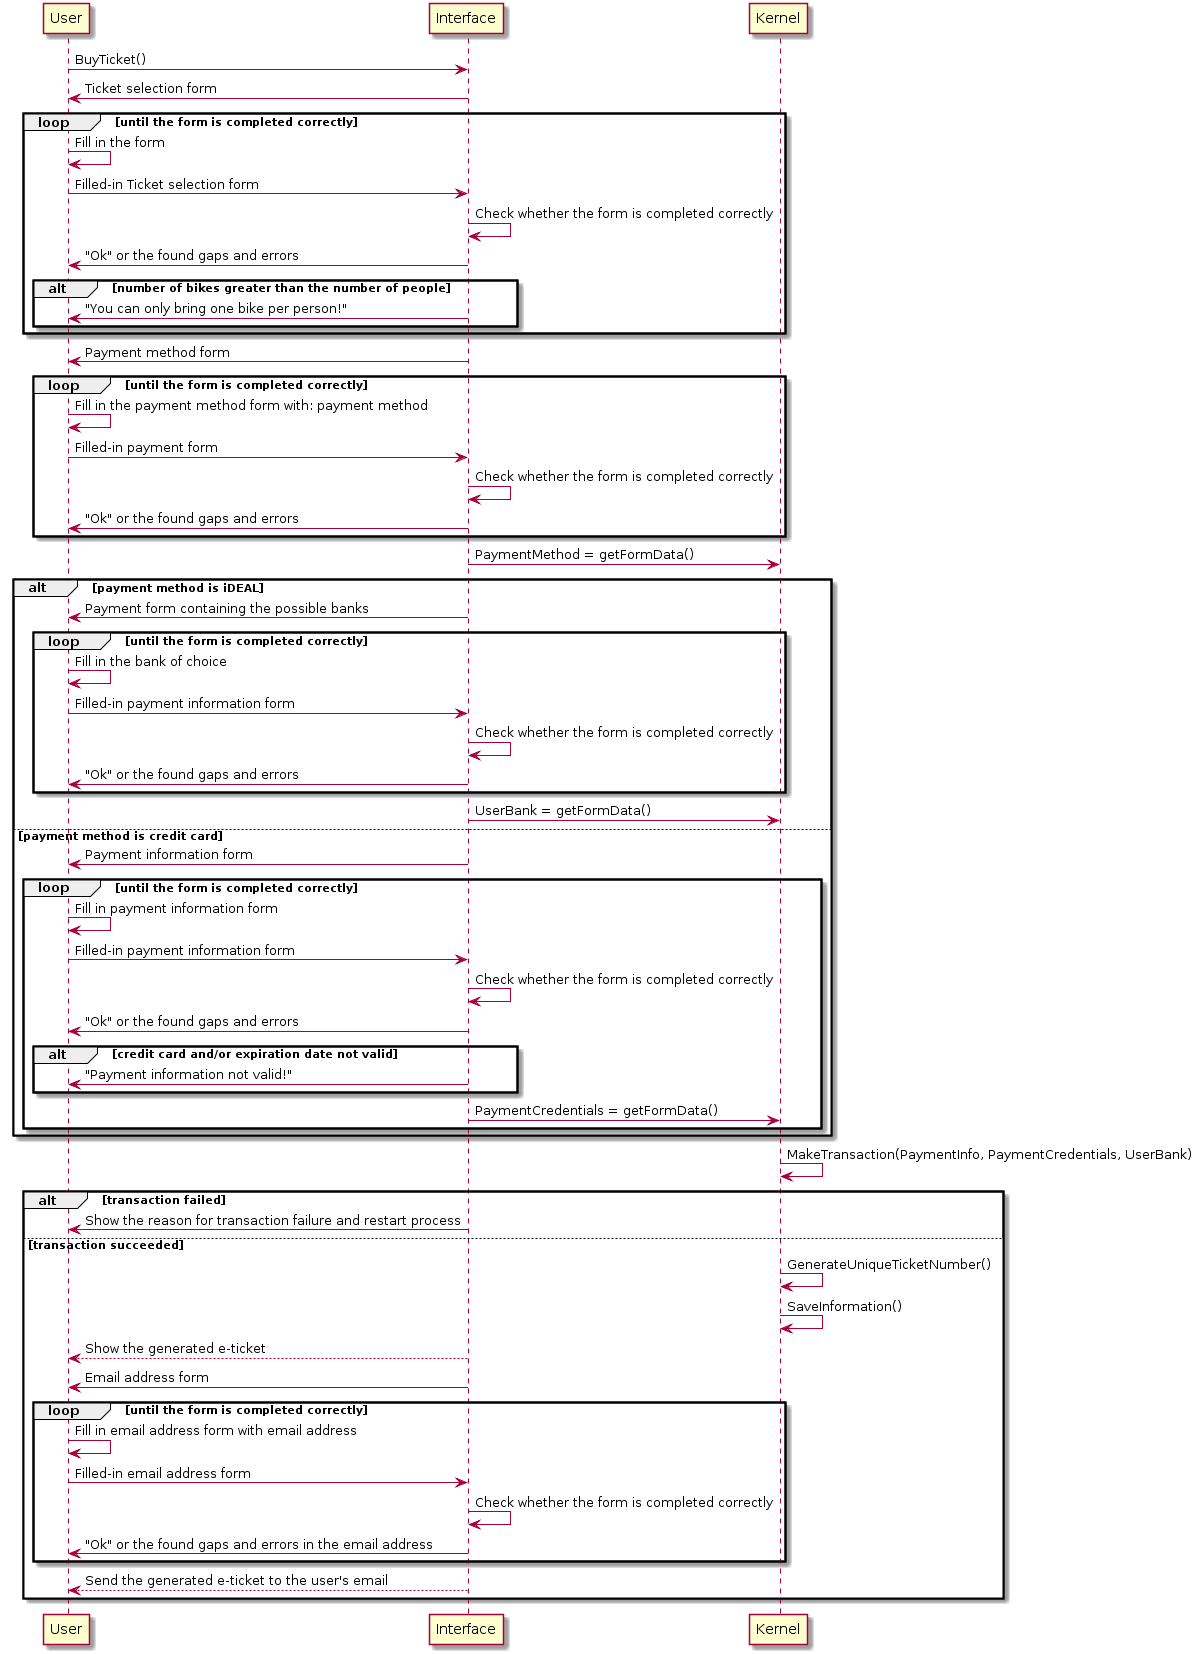
\includegraphics[scale=0.45]{Iteration_3/Files/UC1_gb.png}
\end{lrbox}

\ifdim\ht\mysavebox>\textheight
    \setlength{\myrest}{\ht\mysavebox}%
    \loop\ifdim\myrest>\textheight
        \newpage\par\noindent
        \clipbox{0 {\myrest-\textheight} 0 {\ht\mysavebox-\myrest}}{\usebox{\mysavebox}}%
        \addtolength{\myrest}{-\textheight}%
    \repeat
    \newpage\par\noindent
    \clipbox{0 0 0 {\ht\mysavebox-\myrest}}{\usebox{\mysavebox}}%
\else
    \usebox{\mysavebox}%
\fi

\iffalse \subsubsection{White box SD}
\creator{\studentC}
\updater{\studentA}
\fi

%\includegraphics[scale=0.9]{UC1wb.pdf}



\subsubsection{Design Considerations}
\begin{itemize}
    \item For step 12 and 13a.5 from the Main Success Scenario, no possibilities of errors are possible other than not filling-in the form which is already handled.
    \item For the BB-SD, some annotations were shortened so that the final image would be reasonable in size.
\end{itemize}